%使用xelatex编译
%版权所有,翻版必究
%本文件由程序自动生成,任何修改将被覆盖




%


\subsection{
在Windows平台下搭建开发环境
}\label{s000110}



\subsubsection{
在Windows下安装Qt
}\label{ss000110}


读者可以到 \url{http://download.qt.io/archive/
}
下载最新的Qt运行环境。
然而,遗憾的是,从Qt 5.12.0开始从此网址下载的Qt Windows开发环境并不完整。
%介绍如何下载在线安装包...
读者不得不访问Qt官网 \url{https://www.qt.io
},
注册Qt帐号,然后按照流程下载在线安装包。
不得不说,这对初学者很不友好。
幸运的是,目前Qt网站有一个漏洞。读者可以直接访问
 \url{https://www.qt.io/download-thank-you
},点击“here”下载在线安装包。如\figurename\;\ref{p000000}。

\begin{figure}[ht] %浮动体 here and top ...
\centering %中心对齐
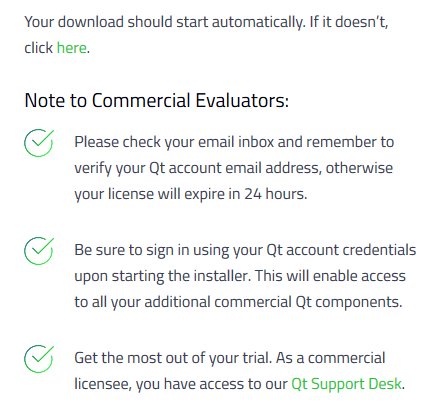
\includegraphics[scale=0.95]{chapter01/windows_download_here.png} %图片路径
\caption{Qt在线安装包下载路径} %标题
\label{p000000} %索引
\end{figure}

以管理员身份运行在线安装包,
选择安装路径时请不要选择包含空格和中文字符的路径。
虽然现代开发环境对于空格和中文字符支持良好,
但是,很多第三方辅助工具未必支持空格和中文字符。
包括本书自带的辅助工具也不保证支持空格和中文。

在Windows平台下,建议读者选择安装“MSVC 2017 64-bit”或以上版
或者
“MinGW 7.3.0 64-bit”或以上版本。
Qt选择5.12.0或以上版本。
安装的时候最好选择安装“Sources”、“Qt Charts”、“Qt WebEngine”以及
“Qt Debug Information Files”这些模块。
在“Tools”选项下组好安装“CDB”以及对应的“MinGW”。
本书建议最小安装如\figurename\;\ref{p000001}。

\begin{figure}[ht] %浮动体 here and top ...
\centering %中心对齐
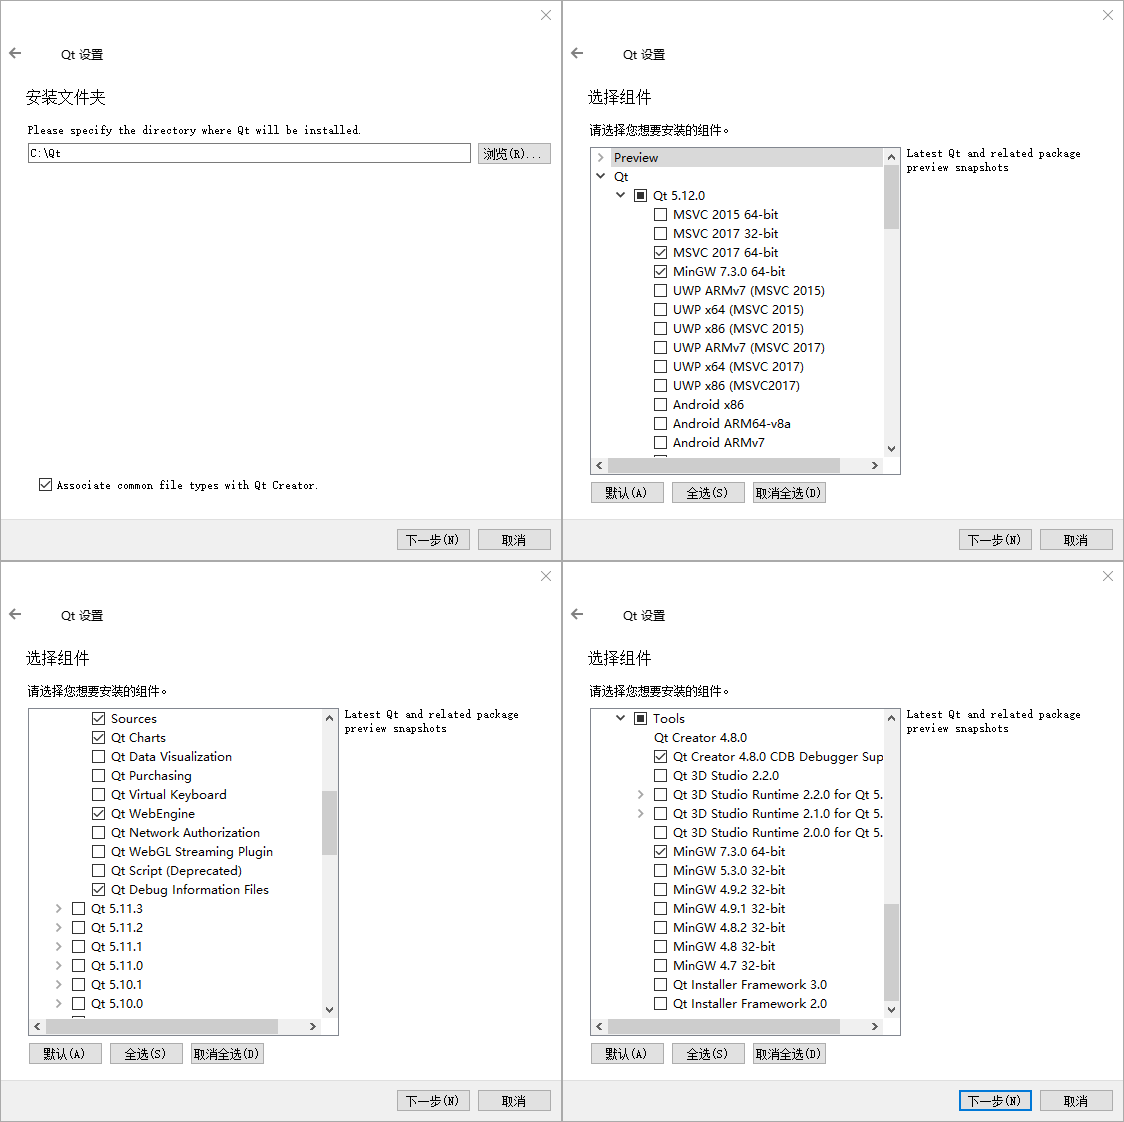
\includegraphics[width=\textwidth]{chapter01/windows_qt_online_install.png} %图片路径
\caption{Qt在线安装建议选择安装组件} %标题
\label{p000001} %索引
\end{figure}



\subsubsection{
在Windows下安装Boost
}\label{ss000210}

读者只需要到 \url{https://www.boost.org
}下载最新Boost稳定版。解压缩,将“boost”文件夹复制到Qt Include路径即可。
比如,
用户的Qt Include路径为\\
“C:\textbackslash{}Qt\textbackslash{}Qt5.12.0\textbackslash{}5.12.0\textbackslash{}msvc2017\_64\textbackslash{}include”,
复制完之后,
应当存在路径\\
“C:\textbackslash{}Qt\textbackslash{}Qt5.12.0\textbackslash{}5.12.0\textbackslash{}msvc2017\_64\textbackslash{}include\textbackslash{}boost”。
当然,读者也可以采用“mklink”建立链接代替拷贝。






%使用xelatex编译
%版权所有,翻版必究
%本文件由程序自动生成,任何修改将被覆盖



